\subsection{Test set 主结果}\label{sec:test}
我们首先检验，在细粒度评分中引入切面条件与局部区域信息，能否改善相同评价条件下的分级表现。在包含 4,107 张图像、240 名患者和 4 个中心的测试集上，完整 VCRE-Fib 取得最低的预设综合风险（$\risk=0.186865$），其后依次为 w/o Weak Loc.（0.191308）、w/o View（0.193799）和 SFibAI（0.201180；表~\ref{tab:main}）。三者相对 SFibAI 的绝对差分别为 $-0.014315$、$-0.009872$ 和 $-0.007380$，对应相对降低 7.115\%、4.907\% 和 3.668\%，均由未取整数值计算。该结果表明，在本次比较中，提供空间输出的三个模型均获得了相对基线的主终点收益，其中联合使用两类空间模块的完整模型表现最好。所有结果来自经验证集选择并冻结的检查点，描述当前测试集上的观测差异。
\inputtable{tab01_main}

\subsection{模块删除比较显示不同的风险改善分布}
为进一步理解上述收益，我们比较两个独立训练的删除变体。保留切面条件化的 w/o Weak Loc.\ 具有更低的 patient-max COR，而保留弱定位的 w/o View 具有更低的 image COR 和 patient-median COR（表~\ref{tab:main}）。这说明两种变体在不同评价层级上的优势并不一致。完整模型则在这些风险指标及中心平衡 COR 上均取得最低值，其综合风险比两个变体中较低的 w/o Weak Loc.\ 再降低 0.004443。因此，联合设计的收益同时体现为主终点降低和跨评价层级的风险改善。该比较反映模型设计的整体表现，尚未分离监督、容量和信息参与方式的影响，也不构成统计优越性或模块协同效应的证明。

\subsection{分级收益同时体现在图像与患者层级}
综合风险的改善伴随着具体评分指标的改善。在图像级，完整 VCRE-Fib 将 SFibAI 的 MAE 从 0.391313 降至 0.377857，四级准确率从 64.11\% 提高至 67.03\%，严重错误率从 9.98\% 降至 9.37\%（表~\ref{tab:image}）。其余图像级指标，包括 RMSE、TMAE、image COR、$\pm0.3$ 与 $\pm0.5$ 准确率及 macro-F1，也均由完整模型取得最优值。这些结果共同表明，当前观测收益覆盖连续评分误差、容差内一致性及四级判别。
\inputtable{tab05_image}

完整模型在 patient-max、patient-median 及中心平衡 COR 上仍取得最低值（表~\ref{tab:main}）。部分阈值准确率由删除变体取得更高值；完整患者级指标及这些差异见附录~\ref{sec:appendix-patient}。

\subsection{分级风险的改善伴随空间任务的取舍}
我们进一步考察，两类空间信息共同参与评分时，其辅助任务表现是否也同步提高。完整 VCRE-Fib 的切面准确率为 66.81\%、macro-F1 为 0.665861、CE 为 0.916542（4,107 张测试集图像）；弱目标 Dice/IoU 为 0.360312/0.235487（4,035 张有效图像；表~\ref{tab:auxiliary}）。相比之下，w/o Weak Loc.\ 的切面准确率和 macro-F1 更高（75.70\% 和 0.757500），w/o View 的 Dice/IoU 更高（0.430661/0.298825）。因此，最低分级风险并未伴随两项空间任务各自最优。完整模型是四者中唯一同时输出评分、切面和定位图的模型，而这一输出完整性伴随着辅助任务表现的取舍。弱目标重叠衡量与局部粗标注的一致性，不代表完整病灶分割。
\inputtable{tab07_auxiliary}

\subsection{联合输出呈现评分与空间判断的分歧}
图~\ref{fig:cases} 展示这些输出能够提供哪些具体的检查信息。四例测试集病例覆盖四种真实切面，每行并列呈现原始超声、医生标注与定位预测，并保留参考/预测评分及完整切面名称。(a)--(c) 展示定位响应与标注的对应；其中 (a) 的评分接近参考值（2.4/2.409），切面却将真实左肋下横切面误判为剑突下矢状切面。该例表明，评分接近并不保证空间判断正确，而联合输出使这类分歧能够被直接查看。

(d) 的参考/预测评分为 1.4/1.491，在固定色标和阈值下呈现超出局部矩形框的响应，附录另列两例验证集示例。框外响应提供了可检查的位置，但既可能对应相关组织，也可能是错误激活，不能据此确认完整病灶覆盖或临床正确性。所有定性病例均由用于定量评价的冻结检查点生成；其作用是展示可检查的信息，不附加医生解释，也不据此主张已验证的临床复核收益。
\begin{figure}[!tb]
\centering
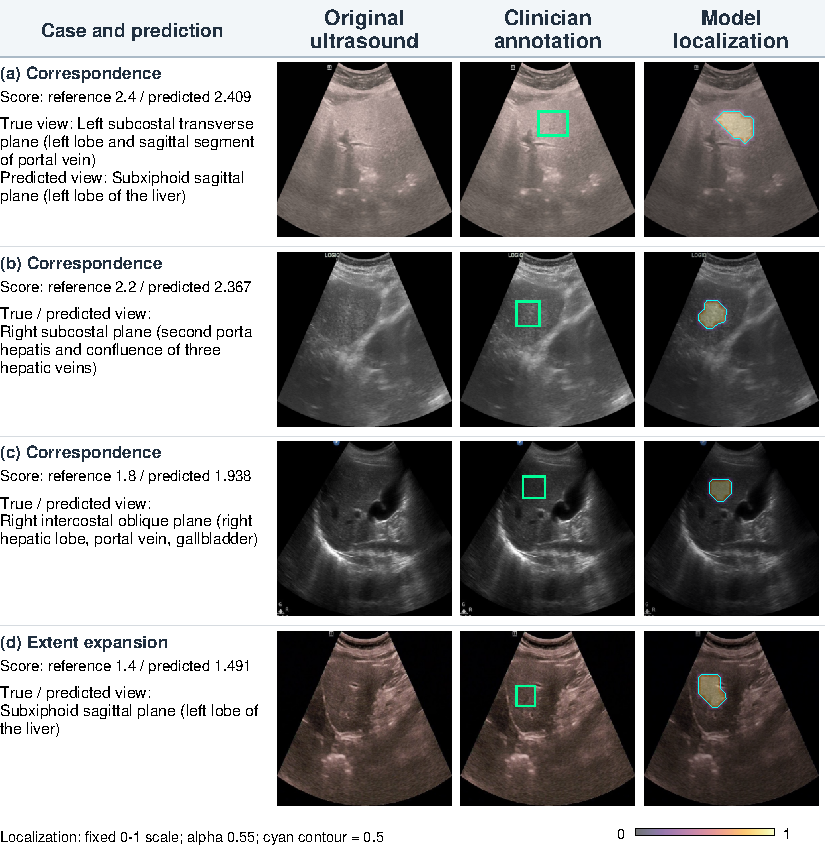
\includegraphics[width=\linewidth]{figures/assets/fig06_cases.pdf}
\caption{\lang{Four selected test cases, with reference and predicted scores and acquisition views at left. Predictions use the frozen checkpoint evaluated quantitatively. Rows (a)--(c) show localization correspondence; (d) shows a response beyond local boxes. Green boxes denote clinician annotations; localization uses a $[0,1]$ scale, opacity 0.55, and a cyan 0.5 contour. In row (a), the predicted view differs from the reference. These selected examples illustrate spatial outputs without establishing population localization performance or complete lesion extent.}{四个筛选的测试集病例，左侧标出参考及预测评分和扫查切面。预测使用参与定量评价的冻结检查点。(a)--(c) 展示定位对应，(d) 展示局部框外响应。绿色框为医生标注；定位色标为 $[0,1]$、透明度为 0.55，青色轮廓阈值为 0.5。(a) 的预测切面与参考切面不同。这些筛选示例用于展示空间输出，不代表总体定位水平或完整病灶范围。}}
\label{fig:cases}
\end{figure}


\subsection{联合预测的计算开销}
我们进一步量化同时提供评分与两类空间输出的计算代价。在同一 A100-SXM4-80GB 上按 FP32 测量，SFibAI、w/o View、w/o Weak Loc.\ 和完整 VCRE-Fib 的 batch-one 中位延迟分别为 5.620、6.171、7.122 和 7.371 ms。完整模型相对 SFibAI 增加 7.81\% 参数、4.24\% 计数 MACs，以及 1.751 ms 中位延迟。附录表~\ref{tab:resources} 同时报告 batch 1 和 8 的延迟、P95 与显存，给出分级和输出收益所对应的资源开销。
